\subsection{Figma Design}\label{figma_design}
\begin{minipage}{0.6\textwidth}
    Zur Erstellung eines Mockup des Designs für die \acs{gui} der \acs{rltanzeige} wurde Figma verwendet. Figma Design ist eine Applikation zum Erstellen von Prototypen im Bereich \ac{uxui}. Dabei kann im Team in Echtzeit zusammen gearbeitet werden. Mit Figma können in das erstellte Design direkt interaktive Funktionen eingebaut werden, um ein realistisches Prototyping zu ermöglichen. Ein weiterer Vorteil von Figma ist der sog. \enquote{Dev Mode}. Mit diesem können Entwickler direkt auf das Design zugreifen und Details finden, die benötigt werden, um das Design in Code umzusetzen. \cite[vgl.][]{figma_design:o.J.}
\end{minipage}%
\hfill
\begin{minipage}{0.37\textwidth}
	\centering	
	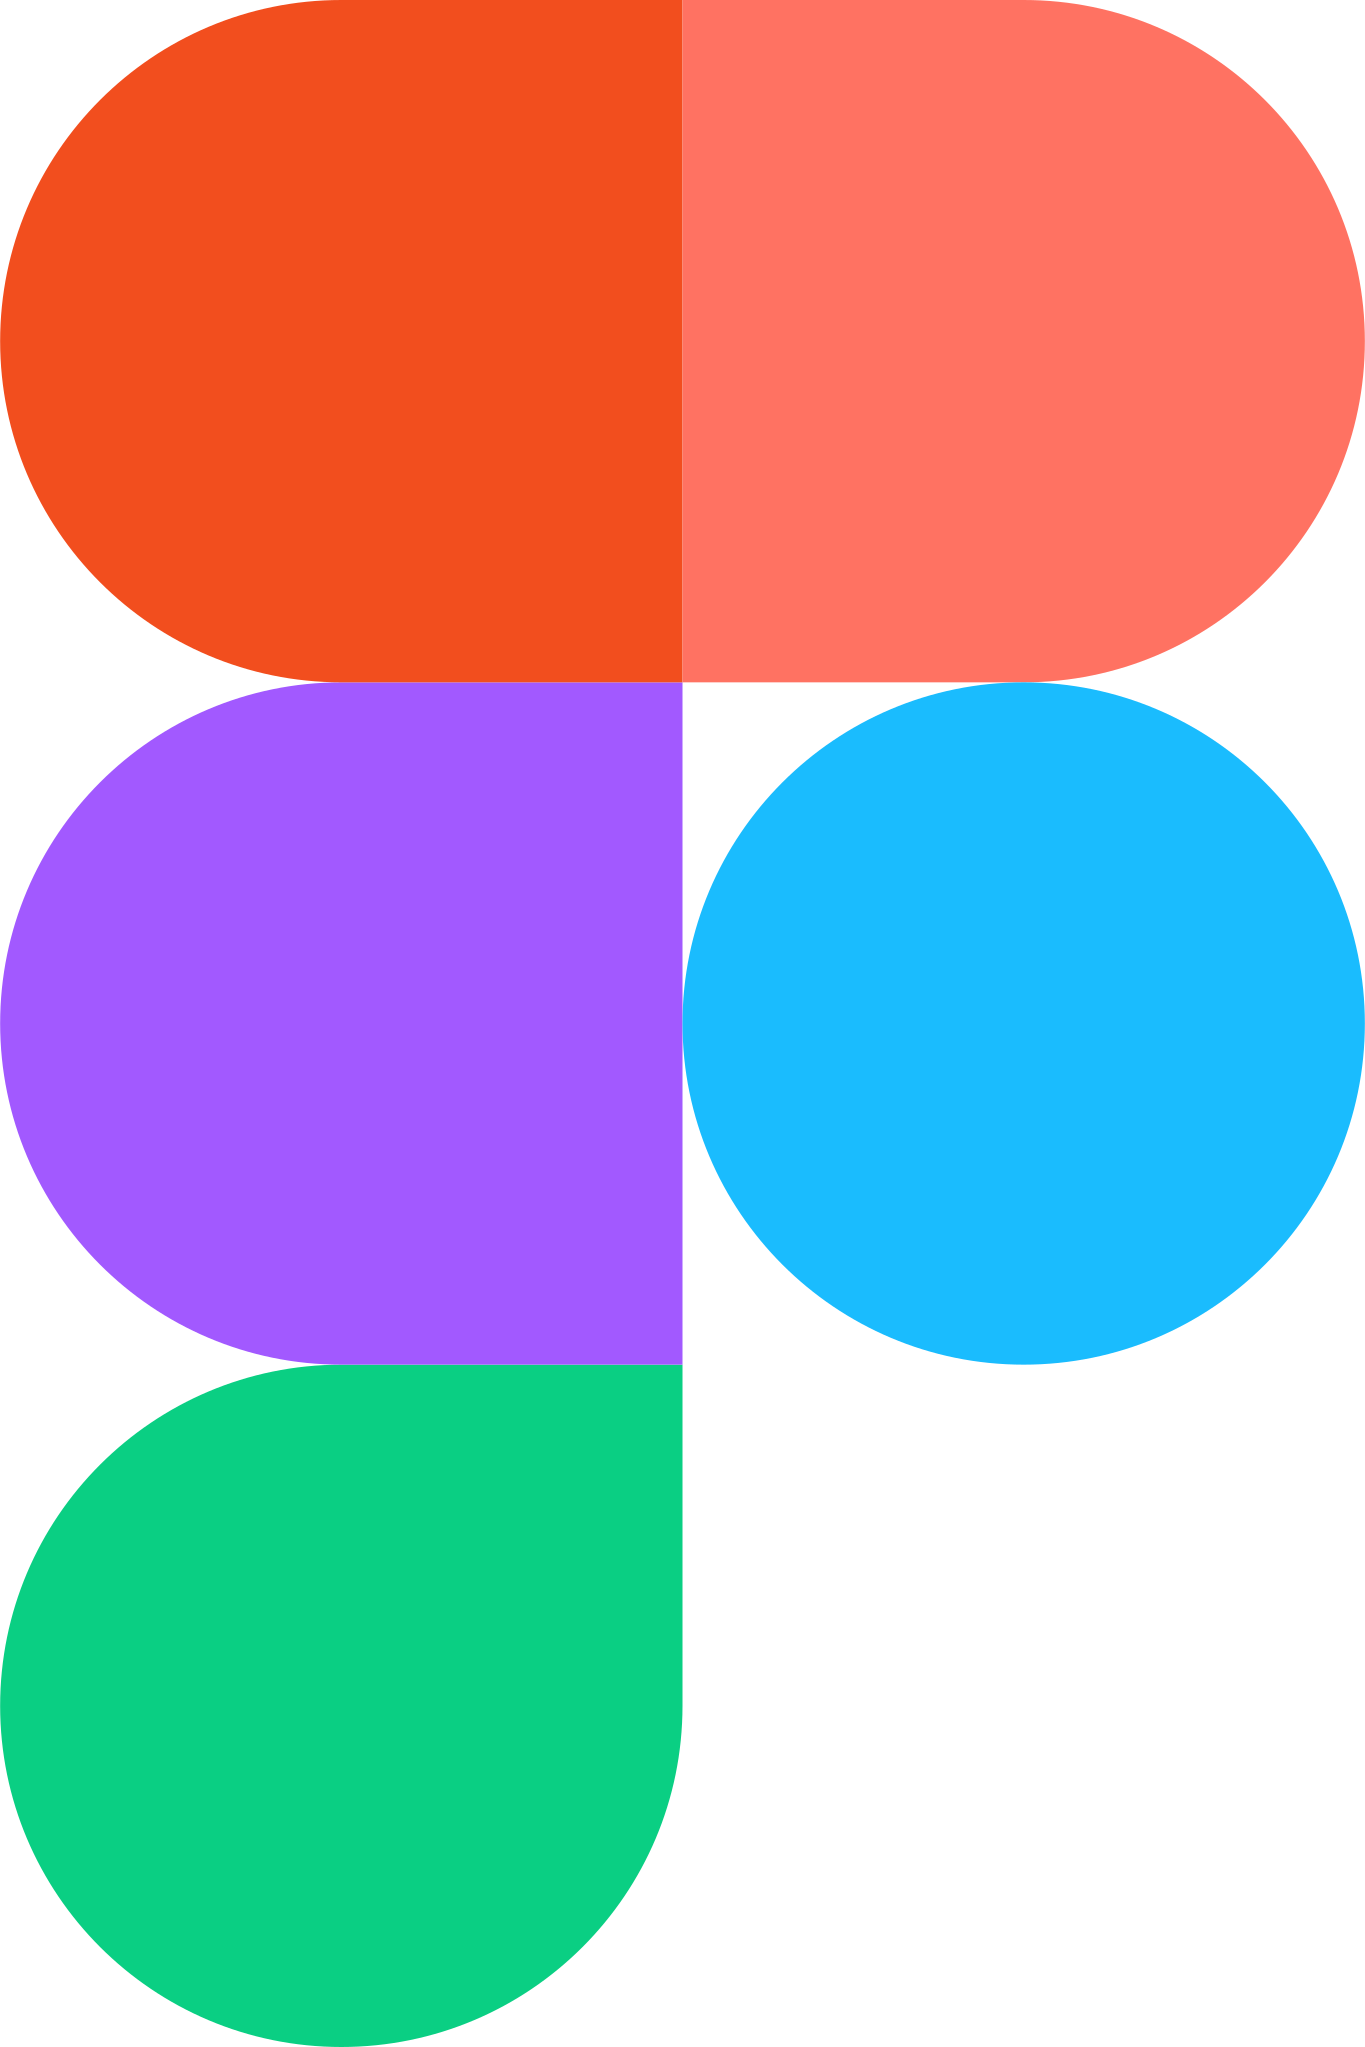
\includegraphics[width=0.50\textwidth]{figma_logo}
	\captionof{figure}{Figma Logo (Quelle: 
		\url{https://en.m.wikipedia.org/wiki/File:Figma-logo.svg}) \label{fig:figma_logo}}
\end{minipage}
\vspace{1ex}

Bei Erstellung des Designs für die \acs{rltanzeige} liegt die Priorität auf Übersichtlichkeit und guter Leserlichkeit. Die Wahl eines $3,5$-Zoll Displays hätte (mit ausreichender Übersichtlichkeit) lediglich die simultane Darstellung von maximal zwei Werten erlaubt. Die tatsächliche Wahl eines $7$-Zoll Displays zur Anzeige ermöglicht hingegen die zeitgleiche Darstellung mehrerer Werte, wobei fünf bis sechs Werte den idealen Kompromiss zwischen genug Information und Übersichtlichkeit bieten. Um die Übersichtlichkeit weiter zu erhöhen ist die Kategorisierung der Messwerte in sinnvolle und zusammenhängende Seiten wichtig. Alle Informationen zu wichtigen Temperaturen sollen beispielsweise auf einer Seite gruppiert sein, während alle Informationen zu einem bestimmten Ventilator auf einer anderen Seite zu finden sind. Hierbei benötigt jede jeweilige Seite eine Überschrift zur Orientierung. Zusätzlich sollte es eine Indikation geben, die der Nutzerin oder dem Nutzer signalisiert, auf welcher Seite sie oder er sich gerade befindet. Tasten zum Seiten wechseln werden nicht benötigt, da an der \acs{rltanzeige} zwei Taster verbaut sind.

\begin{figure}[H]
    	\begin{subfigure}[t]{0.5\textwidth}
    		\centering
    		\frame{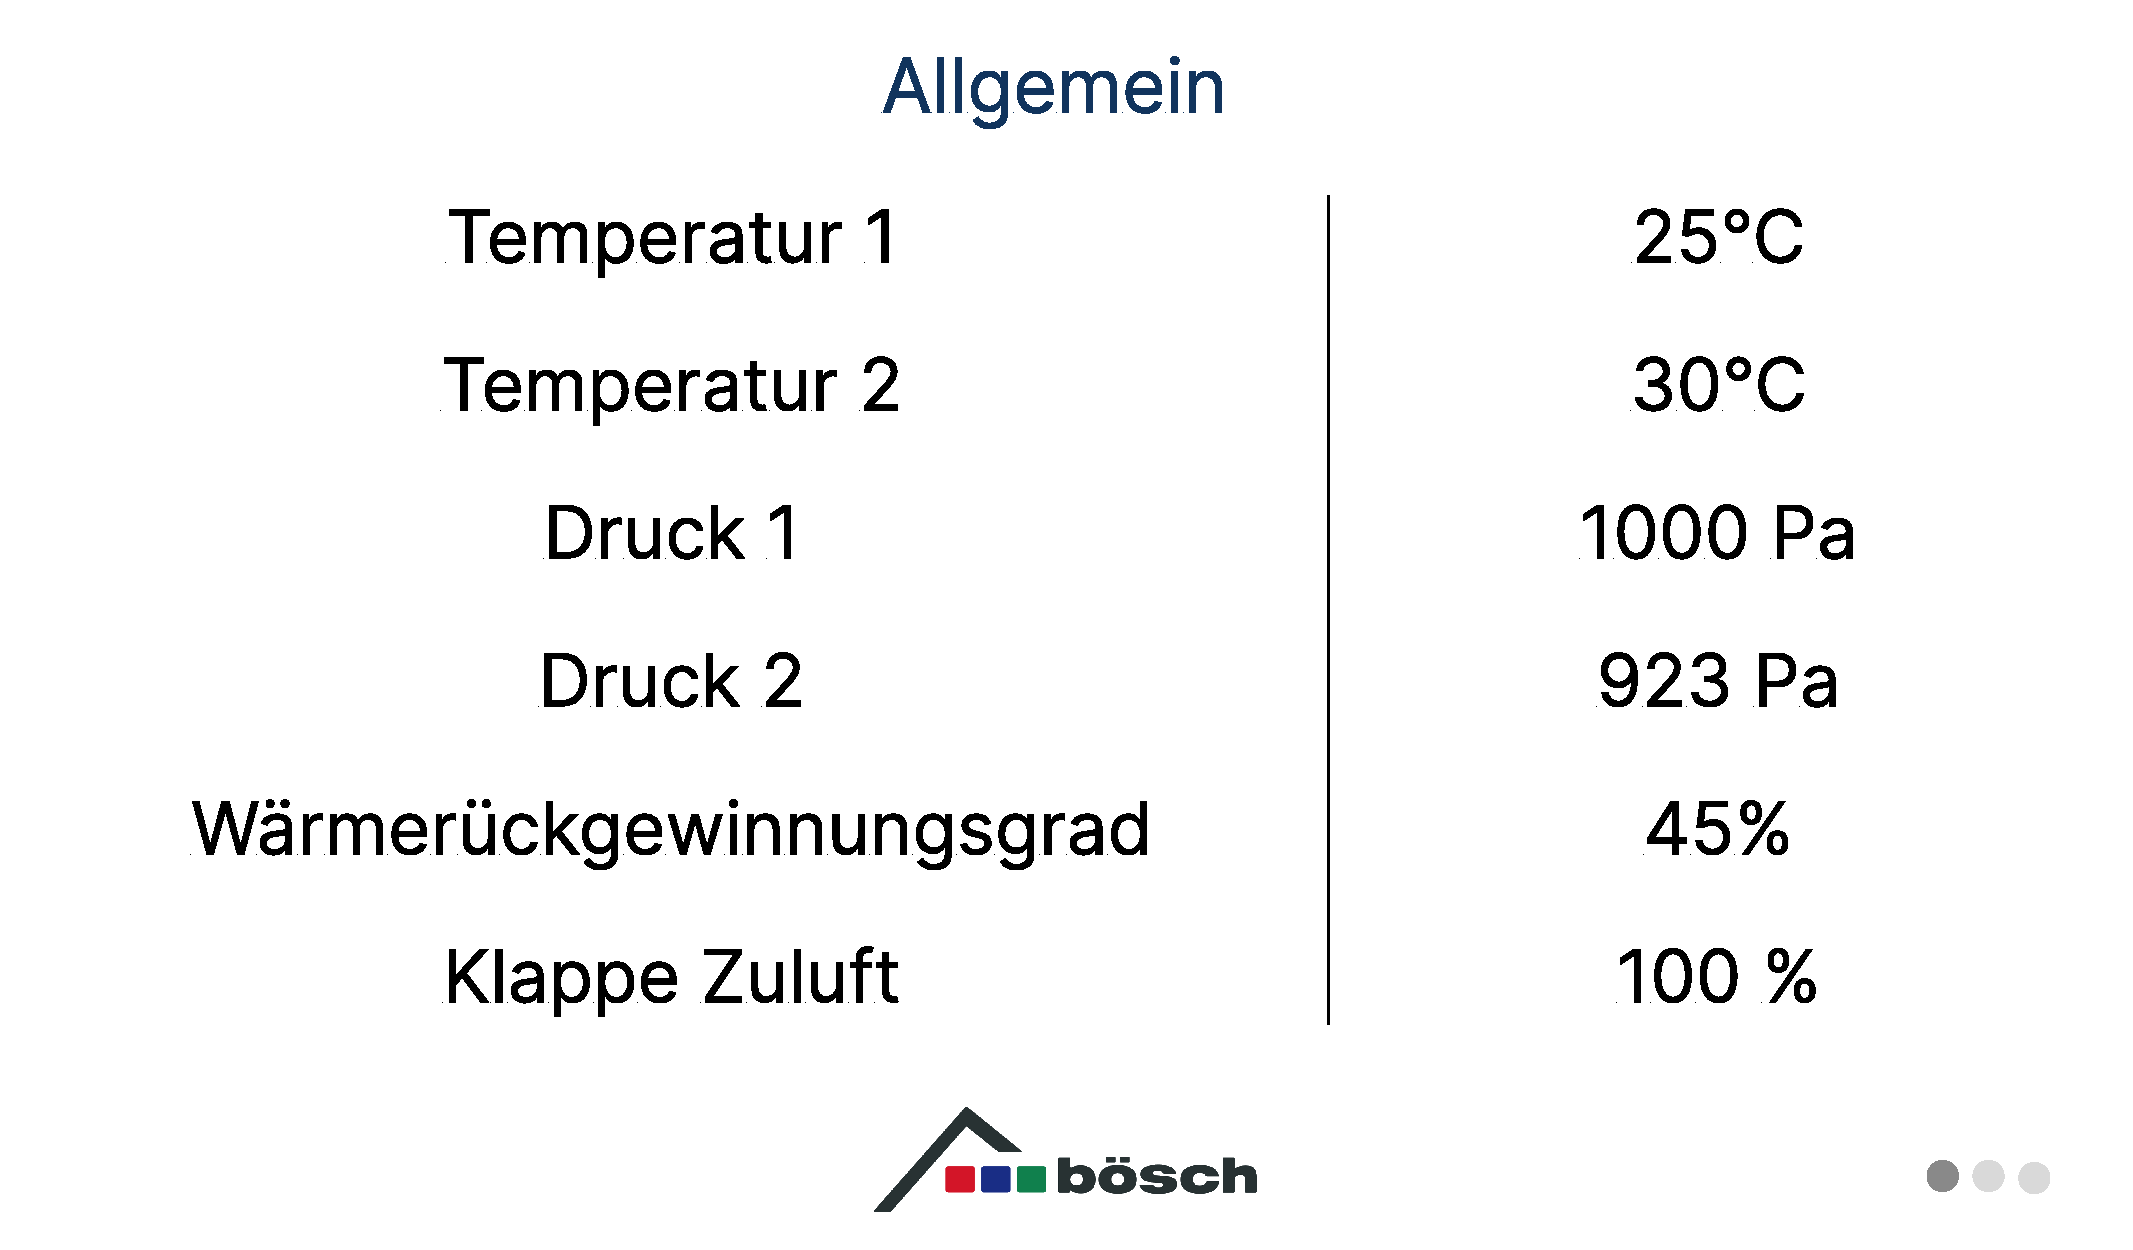
\includegraphics[width=0.99\textwidth, page=1]{design_varianten}}
    		\caption{Design Variante A \label{fig:variante_a}}
    	\end{subfigure}
        \hfill
    	\begin{subfigure}[t]{0.5\textwidth}
    		\centering
    		\frame{\includegraphics[width=0.99\textwidth, page=2]{design_varianten}}
    		\caption{Design Variante B \label{fig:variante_b}}
    	\end{subfigure}
    \begin{subfigure}[t]{\textwidth}
		\centering
		\frame{\includegraphics[width=0.70\textwidth, page=3]{design_varianten}}
		\caption{Design Variante C \label{fig:variante_c}}
	\end{subfigure}
	\caption{\acs{gui} Design Varianten \label{fig:design_varianten}}
\end{figure}

Mit den zuletzt genannten Kriterien wurden drei Designvarianten entworfen (siehe Abb. \ref{fig:design_varianten}). Zur Umsetzung gelangte schlussendlich Variante C (siehe Abb. \ref{fig:variante_c}). Diese bietet mit dem Kontrast im Hintergrund jedes einzelnen Messwerts und der listenartigen Aufzählung die besten Eigenschaften, um Messwerte auf einem Display mit begrenzter Auflösung und Helligkeit in Umgebungen mit suboptimalen Bedingungen ablesen zu können. 

